\documentclass[french,12pt]{article}
\usepackage{babel}

\usepackage[utf8]{inputenc}%encodage des caractères
\usepackage[T1]{fontenc}%encodage de la police
\usepackage{graphicx}
\usepackage{amsmath}
\usepackage{hyperref}
\usepackage{tikz}
\usepackage{listings}
\usepackage[linesnumbered,ruled,french,onelanguage]{algorithm2e} 
\setlength{\parindent}{0pt} 
\makeatletter
\g@addto@macro{\@algocf@init}{\SetKwInput{KwOut}{Sortie}}
\makeatother

\title{Rapport Projet 2}

\date{07 Avril 2023}

\begin{document}

\maketitle
\rule{\linewidth}{.5pt}

\begin{figure}[h]
	\begin{center}
		
\includegraphics[scale=0.8]{img/fond.png}	
	\end{center}
\end{figure}
\rule{\linewidth}{.5pt}
\begin{center}
\author{Antonin MONTAGNE-21901206\\ Lou-Anne GAUTHERIE-22001251\\ Nathan SAKKRIOU-22003438 \\
    Yanis HABAREK-22010593}
\end{center}

\begin{figure}[b]
	\begin{center}
		
\includegraphics[scale=0.7]{img/unicaen.png}	
	\end{center}
\end{figure}

\thispagestyle{empty}
\setcounter{page}{0}
\newpage

\tableofcontents
\newpage

\section{Introduction}

\subsection{Plan du rapport}

Nous évoquerons d'abord quels étaient nos objectifs de départ (\ref{objectifs}), puis nous détaillerons les différentes étapes de la création de notre projet avec les rôles de chacuns (\ref{organisation}). Ensuite nous présenterons l'architecture de ce projet (\ref{architecture}), ainsi que les éléments techniques utilisées (\ref{elemTech}) dans notre code. Finalement nous présenterons certaines expérimentations (\ref{experim}) et terminerons par une courte conclusion (\ref{conclusion}).

\subsection{Objectifs du projet} \label{objectifs}

Nous avions pour but de créer une application d'analyse d’identité d’auteurs et détection de plagiat. Certaines contraintes nous étaient données :
\begin{itemize}
	\item Créer un corpus d'entraînement et de test.
	\item Traiter ce corpus pour en obtenir une représentation appropriée.
	\item Mettre en oeuvre un ou plusieurs classificateurs.
	\item Évaluater les performances des classificateurs par rapport au
	rappel et à la précision.
	\item Intégrer des caractéristiques supplémentaires dans le processus.
\end{itemize}

\section{Fonctionnalités implémentées} \label{organisation}

\subsection{Description des fonctionnalités}

Cette application possède une page web en tant qu'interface graphique. Cette page web est chargée via une API pour que les documents communiquent directement entre eux et que l'analyse de plagiat charge en temps réel.\\

Il suffit de lancer l'API dans un terminal, et le terminal donne l'adresse du serveur à rejoindre o\\

Sur cette page web se trouve une fonctionnalité pour comparer le document du client, avec ceux du corpus. Le client peut d'abord découvrir les similarités entre son document et les autres (mots revenants fréquemment), puis il peut ensuite voir les auteurs de ces documents.\\

La deuxième fonctionnalité  de la page est la comparaison de deux documents. Le client choisit les deux documents à comparer, mais également l'algorithme utilisé.

Une fois la sélection effectuée, les données sont envoyées à l'API, qui charge les fonctions correspondantes.

\subsection{Organisation du projet}

Pour commencer, Nathan s'est occupé de créer tout le corpus d'article en scrappant les archives de Libération. Il s'est également occupé de la création d'un interface permettant de manipuler les articles stocké dans notre base de donnée et pour finir il s'est occupé de l'implémentation des algorithmes avec l'API.\\

Pendant ce temps, Yanis et Antonin se sont occupés des algorithmes. Antonin a codé l'algorithme de classification \textit{Bayes} et Yanis les algorithmes de comparaison \textit{Jaccard}, \textit{Difflib} et  \textit{Vecteur Cosinus}.\\

Dans le fichier \texttt{Bayes.py}, nous retrouvons une classe \texttt{Bayes} qui contient plusieurs fonctions pour manipuler le contenu d'un fichier:
\begin{itemize}
	\item \texttt{countClass} compte le nombre de fois où une classe
	apparait dans le corpus.
	\item \texttt{countOccurenceWordsClasse} compte le nombre de fois où un
	mot apparait dans une classe.
	\item \texttt{countWordClasse} compte le nombre de mots dans un classe.
	\item \texttt{countWordDifferent} compte le nombre de mots différents
	dans le corpus.
	\item \texttt{chooseClass} calcule l'auteur qui est le plus susceptible
	d'avoir écrit le texte.
	\item \texttt{recall} calcule l'efficacité du classificateur.
	\item \texttt{precision} calcule la précision du classificateur.\\
\end{itemize}
Le fichier \texttt{difflib$\_$algo.py}  contient la classe \texttt{Difflib} qui comprend:
\begin{itemize}
\item la fonction \texttt{compare} qui prend en argument deux fichiers .txt et qui les compare grâce à la classe \texttt{difflib} de python.\\
\end{itemize}
Le fichier \texttt{jaccard.py} contient la classe \texttt{Jaccard} qui comprend :
\begin{itemize}
    \item la fonction \texttt{compare} qui compare cette fois ci deux fichiers .txt  en utilisant leur taille, leur intersection et leur union.\\
\end{itemize}


Le fichier \texttt{techniques$\_$vecteurs$\_$cosinus.py} contient la classe \texttt{VecteurCos} qui comprend:
\begin{itemize}
    \item La fonction \texttt{cosine$ \_$similarity} qui prend en argument deux string, elle créée ensuite un vecteur de mots pour chaque texte puis utilise la fonction \texttt{set} de python pour supprimer les doublons.\\

\end{itemize}

De son coté, Lou-Anne a créé l'API (codé en python) et la page web (html, css, js). Elle a implémentée des éléments \texttt{input-file} qui ouvre un explorateur de fichiers pour pouvoir choisir un fichier, et des éléments \texttt{button} et \texttt{select} pour sélectionner la comparaison et l'algorithme voulu. \\
Ces données sont stockées dans des dictionnaires \texttt{dict1} et \texttt{dict2} (codé en javascript) et ceux-ci sont envoyés à l'API via la méthode \texttt{post}. C'est ensuite cette même API qui gère les données.

\section{Architecture du projet} \label{architecture}

\subsection{Diagrammes des modules et des classes}

Diagramme de tous les packages (et leurs dépendances):

\begin{center}
	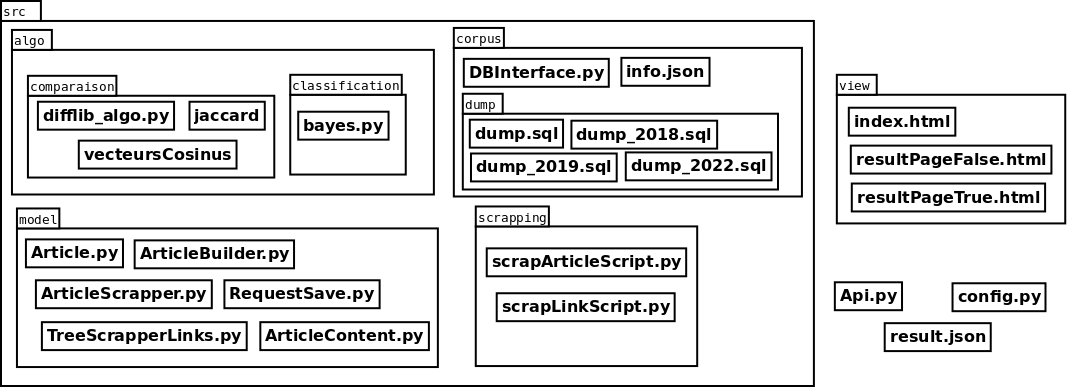
\includegraphics[scale=0.3]{img/DiagrammeClasse.png}	
\end{center}


\subsection{Paquetages utilisées}

Nous avons utilisé plusieurs classes de Python nécessaires au lancement de l'application et à l'analyse de documents :

\begin{table}[h]
   \begin{tabular}{| c | c | c |}
      \hline
      \textbf{noms des classes} & \textbf{utilité} & \textbf{emplacement} \\
      \hline
      fastapi & framework permettant de simplifier la création d'api & Api.py\\
      \hline
      psycopg2 & intéraction avec base de & DBInterface.py \\
      & données PostgreSQL & \\
      \hline
      path & manipulation des chemins de  & scrapArticleScript.py \\
      & fichiers et de répertoires & scrapLinkScript.py \\
      \hline
      sys & accès à des fonctionnalités & scrapArticleScript.py \\
      & spécifiques au système d'exploitation & scrapLinkScript.py \\
      & & Bayes.py \\
      \hline
      math & fournit des fonctions mathématiques & Bayes.py \\
      \hline
      os & accès à des fonctionnalités pour interagir & difflib $\_$algo.py \\
      & avec le système d'exploitation sous-jacent & \\
      \hline
      difflib & fournit des fonctions pour comparer  & difflib$\_$algo.py
      \\ & et différencier des séquences de texte & \\
      \hline
   \end{tabular}
   \caption{Liste des classes Python utilisées}
\end{table}

\section{Éléments techniques} \label{elemTech}

\subsection{Corpus d'article}

Le corpus est une partie très importante de notre projet car c'est grâce aux informations qu'il contient que l'algorithme de classification (bayes dans notre cas) va pouvoir attribuer le texte fourni en entrée a tel ou tel auteur.\\

\subsubsection{Structure du corpus}

Comment ce matérialise t'il : Nous avons fait le choix d'utiliser une base de donnée relationnelle, PostgreSQL. Cette base de donnée contient 2 tables :\\

\begin{itemize}
    \item researched\_table : qui va nous permettre de stocker les urls des articles que nous voulons scrapper (inutile dans l'utilisation finale mais très importante pour la création du corpus). | \textit{id SERIAL, year VARCHAR, month VARCHAR, day VARCHAR, url VARCHAR}

    \item articles\_table : qui va nous permettre de stocker le contenu des articles et leurs auteurs. C'est les informations de cette table qui sera utilisé par notre algorithme de classification. | \textit{id SERIAL, author TEXT, text\_article TEXT}
\end{itemize}

\subsubsection{Création du corpus}

La création de notre corpus se passe en 2 étapes : \\
\begin{itemize}
    \item 1 : Récupération d'articles
    \item 2 : Scrapping du contenu de ces articles et de leurs auteurs\\
\end{itemize}

Étape 1 : \\\\
Pour remplir notre corpus, nous avons fait un choix dès le début de notre projet.\\
Il nous fallait des articles et les auteurs associés en quantité de préférence. Pour trouver ce genre d'informations nous nous somme orienté vers des sites de journaux, dans notre cas Libération a été notre premier choix. Libération possède une section archive qui contient les articles paru de 1998 à 2023. Cette section archive est composé de manière très simple. Pour accéder aux articles paru le 23 Mai 2009 (un exemple au hasard), le site nous offre l'URL suivante \hyperlink{https://www.liberation.fr/archives/2009/05/23/}{https://www.liberation.fr/archives/2009/05/23/}. On se rend compte qu'il très facile d'itérer sur toutes les urls. Il suffit simplement de connaître le calendrier des jours que l'on souhaite. Cette information est facilement accessible grâce a la bibliothèque Python \textit{calendar} et la fonction \textit{monthrange}. Grâce a cette fonction nous pouvons savoir combien de jour il y avait en fonction d'une année et d'un mois donné. La génération des URL est théoriquement complétée, en pratique, nous avons crée 4 types d'objet : \textit{LiberationScrapper}, \textit{Year}, \textit{Month} et \textit{Day} :\\

\begin{itemize}
    \item LiberationScrapper est la classe permettant de lancer le processus de création des URL sur une tranche d'année afin d'automatiser au mieux notre processus.\\
    \item Year, Month et Day permettent de générer les valeurs correspondante et des les concaténer à la base de l'URL de Libération. La spécificité de Day, c'est qu'il lance le début du scrapping.\\
\end{itemize}

Nous n'avons pas encore précisé ce que nous renvoyais une URL du type : \hyperlink{https://www.liberation.fr/archives/2009/05/23/}{https://www.liberation.fr/archives/2009/05/23/}. Nous obtenons une liste de lien menant aux articles voulu. Avec les bibliothèques \textit{BeautifulSoup (bs4)} et \textit{Request} il est facile de faire une requête GET pour obtenir la page avec le lien qu'on a créer et de manipuler son DOM. La méthode de la classe Day qui s'occuper de cela est \textit{scrapLiberation(url)}.\\
Une fois tous les liens des articles du jour voulu récupéré, nous les envoyons dans la base de donnée grâce un objet nommé \textit{ScrapDatabase} qui nous permet de faire l'interface entre notre code et notre PostgreSQL, cette classe possède toutes les méthodes nécessaires pour l'insertion de donnée dans chacune de nos tables mais aussi pour récupérer et utiliser les informations nécessaires pour la classificateur (nous utilisons la bibliothèque \textit{psycopg2} pour faciliter la connexion avec une instance postgresql en python).\\\\

Pour résumer cette étape 1 :\\
\begin{itemize}
    \item 1 : Nous avons détecter un pattern simplement utilisable dans les archives de Libération pour accéder a une grosse quantité d'article \textit{https://www.liberation.fr/archives/annee/mois/jour}\\
    \item 2 : Nous avons créer des classes afin d'automatiser la création de ces URL\\
    \item 3 : Nous scrappons les liens des articles et les stockons dans une table de notre corpus.\\
\end{itemize}

Le script qui nous permet d'effectuer toutes ces actions est \textit{scrapLinkScript.py}\\\\


Étape 2 : \\

Nous avons désormais notre table \textit{researched\_table} remplie d'une liste d'URL correspondant a des articles. L'objectif maintenant est de les récupérer, les lire et récupérer le contenu de l'article et l'auteur pour ensuite le stocker dans le corpus.\\

Pour cela nous introduisons quelques nouveaux objets : \\

\begin{itemize}
    \item Article : Représente un Article avec sa date et son URL\\
    \item ArticleContent : Représente un article concret avec son auteur et son contenu\\
    \item ArticleBuilder : Un builder permettant de transformer les données brutes (sous forme de liste de liste de string) récupérés de la base de donnée en Article\\
    \item ArticleScrapper : Permet de scrapper l'URL d'un Article et de le transformer en ArticleContent\\
\end{itemize}

Toutes ces classes sont manipulés dans le script \textit{scrapArticleScript.py} qui permet de sélectionner une année et de scrapper tous les articles correspondant pour ensuite insérer les informations récupérés dans la bonne table du corpus.\\

Le déroulement de cette étape est le suivant : \\

\begin{itemize}
    \item 1 : Récupérer une année précise, (dans notre cas nous avons fait le choix de ne récupérer que les liens d'articles de 2018, 2019, 2021 et 2022) grâce au passage de paramètre d'un script python.\\

    \item 2 : Récupérer les URLs d'articles correspondant dans le corpus et les transformer en une liste d'Articles dans notre code.\\

    \item 3 : Itérer sur cette liste d'Articles et scrapper leur contenu. Il existe une petite subtilité dans cette étape. Certains articles ne sont pas complètement accessible gratuitement, il nous a fallu détecter lesquels l'était afin de ne pas les stocker dans le corpus. Pour cela nous avons detecter la balise CSS qui correspondait a la bannière représentant le besoin d'être premium pour lire cet article et si elle existait sur cette page, alors nous générons un ArticleContent d'erreur, avec des valeur facilement reconnaissable, qui seront filtré avant d'intégrer le corpus.\\

    \item 4 : Une fois avoir scrapper l'ensemble des URLs, nous avons a notre dispositions une liste d'ArticleContent, que nous venons insérer dans la base de donnée (avec l'interface ScrapDatabase) et filtrant les ArticleContent d'erreur.\\
\end{itemize}

A partir de ce moment, il ne suffit plus qu'a scrapper l'intégralité des liens d'articles de notre table articles\_table afin d'obtenir notre corpus.\\

Nous avons rencontré certains problème, comme l'encodage de certains caractere qui ne correspondait pas forcément a ceux accepté par notre base de donnée. Nous avons réussi a surmonter ce problème en faisant en sorte de remplacer les caracteres problèmatique par leurs homologues ascii mais également en modifiant l'encodage de notre corpus.\\


\subsection{API}

Nous avons fait le choix de créer une API comme moyen d'interaction avec notre programme pour le rendre utilisable sans connaissance technique, et simplement. L'idée originale était de la déployer sur VPS, mais nous avons eu quelques problème pour l'accessibilité des ports sur certaines requêtes. Sur la forge, l'api est utilisable en local et parfaitement fonctionnelle.\\

Pour rentrer dans l'aspect nous avons une interface web permettant d'utiliser nos algorithmes de classification et comparaison. Un résultat nous est renvoyé. Pour rentrer cette fois dans la partie programmation nous retrouvons 3 endpoints : \\
\begin{itemize}
    \item "/" [GET] : Pointe sur notre interface de choix d'algo.\\
    \item "verif" [POST] : Requête envoyé par l'utilsateur grâce a la page pointé par le endpoint "/", il nous envoyé les modalités voulu (algorithme, similarité, auteur, fichiers ...), avec ces informations, l'api effectue les instructions correspondantes et inscrit le résultat dans un fichier \textit{result.json}.\\
    \item "/comparaison" [GET] : Affiche le résultat du la demande de l'utilisateur.\\
\end{itemize}

Nous avons utiliser le framework fastapi qui nous permet de facilement utiliser tous les élément pour créer une api également couplé a jinja2, un moteur de templating, qui nous permet de rendre nos page html dynamique en fonction des paramètres qu'on lui fourni à l'envoi du html.

\subsection{Description des algorithmes}

\begin{algorithm}[H]
\DontPrintSemicolon
\KwIn{Un texte (par défaut vide), option (par défaut 0)}
\KwOut{L’auteur qui a le plus de probabilité d'avoir écrit le texte t}
$proba \gets $ dictionnaire vide\;
\For{$auteur \gets corpus$} {
  $proba[auteur] = nbTexteAuteur / nbTexteCoropus$\;
  \For{$mots \gets texte$} {
    \If{$mots $ \textbf{apparaît dans} $texteAuteur$} {
      $proba[auteur] += log(($nb de fois $mots$ dans $texteAuteur+1)
      (nbMotsTextesAuteur + nbMotsCorpus))$\;
   	}
   	\Else {
   	  $proba[auteur] += log(1 / nbMotsTextesAuteur + nbMotsCorpus))$\;
   	}
  }
}
\If{$option$ == 1} {
  \Return{$max(proba, key=proba.get)$}
}
\Return{$phrase + max(proba, key=proba.get)$}
\caption{{\sc Bayes} classifie un ensemble d'observations selon des sacs de mots}
\end{algorithm}



\begin{algorithm}[H]
\DontPrintSemicolon
\KwIn{2 fichiers texte $A$ et $B$}
\KwOut{Probabilité de similarité des fichiers $A$ et $B$}
$A =$ set(A.split())\\
$B =$ set(B.split())\\
\Return{$\frac{|A \cap B|}{|A \cup B|}$}
\caption{{\sc Jaccard} compare deux fichiers grâce à la taille de leur unions, et de leur intersections}
\end{algorithm}

\quad

\begin{algorithm}[H]
\DontPrintSemicolon
\KwIn{2 fichiers texte $A$ et $B$}
\KwOut{Probabilité de similarité des fichiers $A$ et $B$}
$vecteurA =$ fichier $A$ transformé en vecteur\;
$vecteurB =$ fichier $B$ transformé en vecteur\;
\Return{$\frac{vecteurA . vecteurB}{||vecteurA|| . ||vecteurB||}$}
\caption{{\sc Vecteur cosinus} compare deux fichiers en les transformant en vecteur}
\end{algorithm}


\begin{algorithm}[H]
    \caption{{\sc Difflib} est une classe Python qui a été importée  et qui se base sur l'algorithme de Levenshtein.}
    $similarity =$ difflib.$SequenceMatcher$(None,text1,text2).ratio()
\end{algorithm}

	\begin{center}
     	\begin{figure}[h]
     		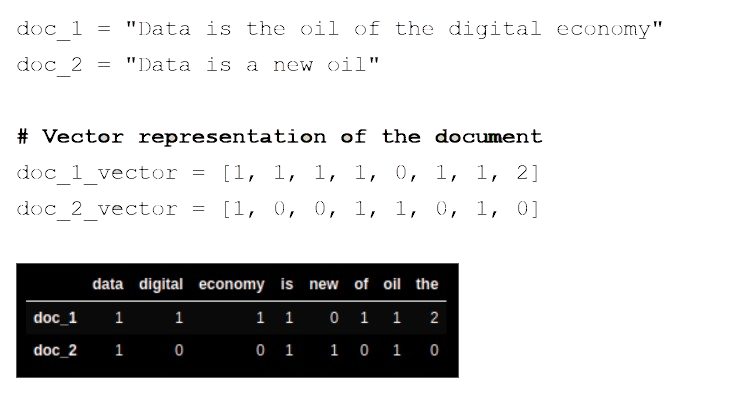
\includegraphics[width=10cm]{img/cos_ex.png}
             \caption{cosinus}
     	\end{figure}
    \end{center}
   		\begin{center}
    		\begin{figure}[h]
    			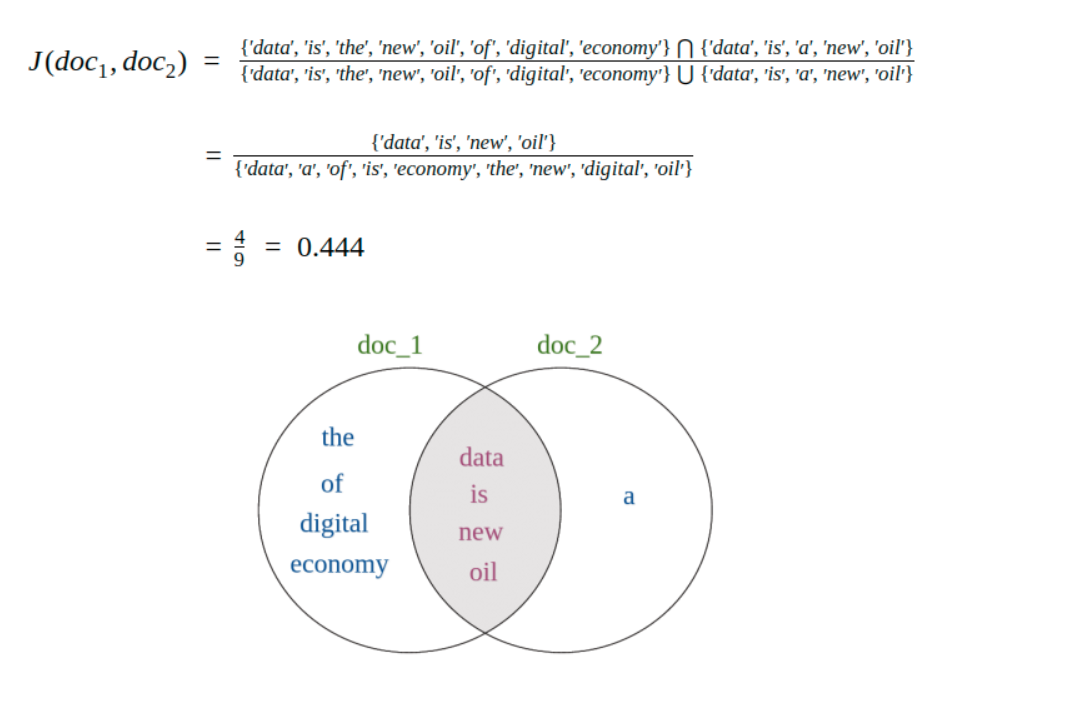
\includegraphics[width=11cm]{img/jaccard_ex.png}
    			\caption{jaccard}
    	\end{figure}
           
          
        \end{center}

\newpage
\section{Expérimentations} \label{experim}
\subsection{Classification}

Grâce aux méthodes recall et précision de la classe \texttt{Bayes}, nous avons lancé plusieurs fois le classificateur de Bayes en faisant varier la taille du corpus d'entraînement et la taille du corpus de test. Comme les résultats du classificateur peuvent varier d'une exécution à l'autre du fait que les corpus soit régénérer à chaque nouvelle instance de la classe Bayes. Nous avons décider de lancer l'algorithme 10 fois de suite avec les mêmes paramètres afin d'obtenir une moyenne.
Voici les résultats obtenu :
\begin{center}
\begin{figure}
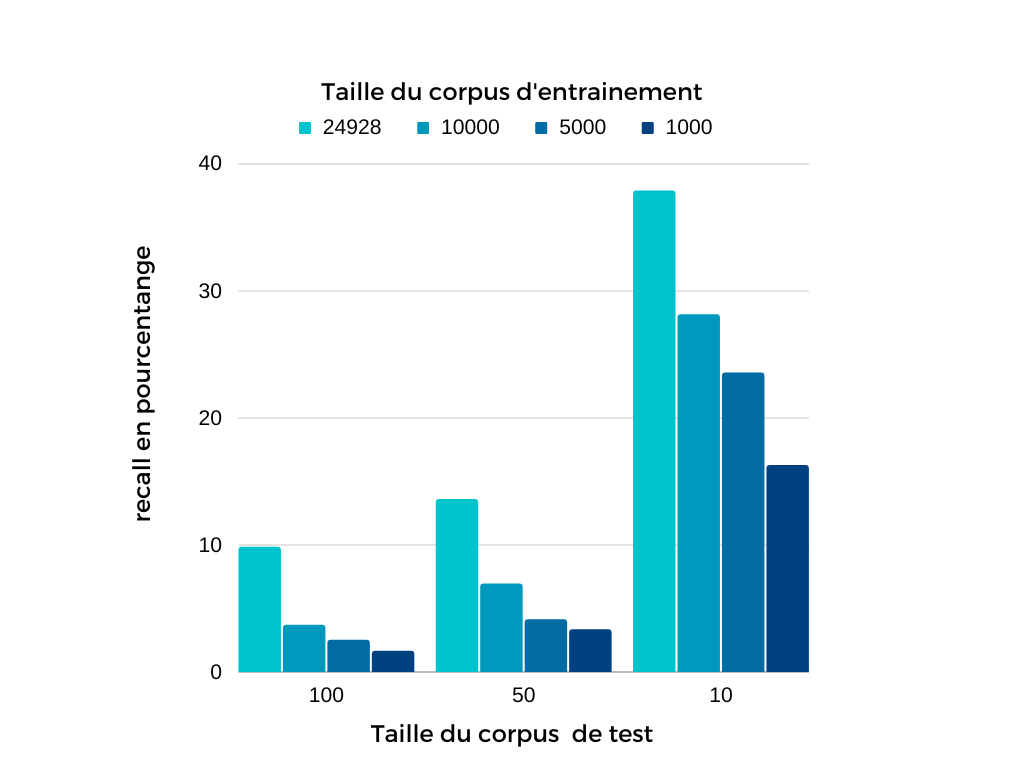
\includegraphics[scale=0.4]{img/TableauRecall.png}
\caption{Graphique de l'efficacité du classificateur}
\end{figure}


\end{center}
\begin{center}
\begin{figure}
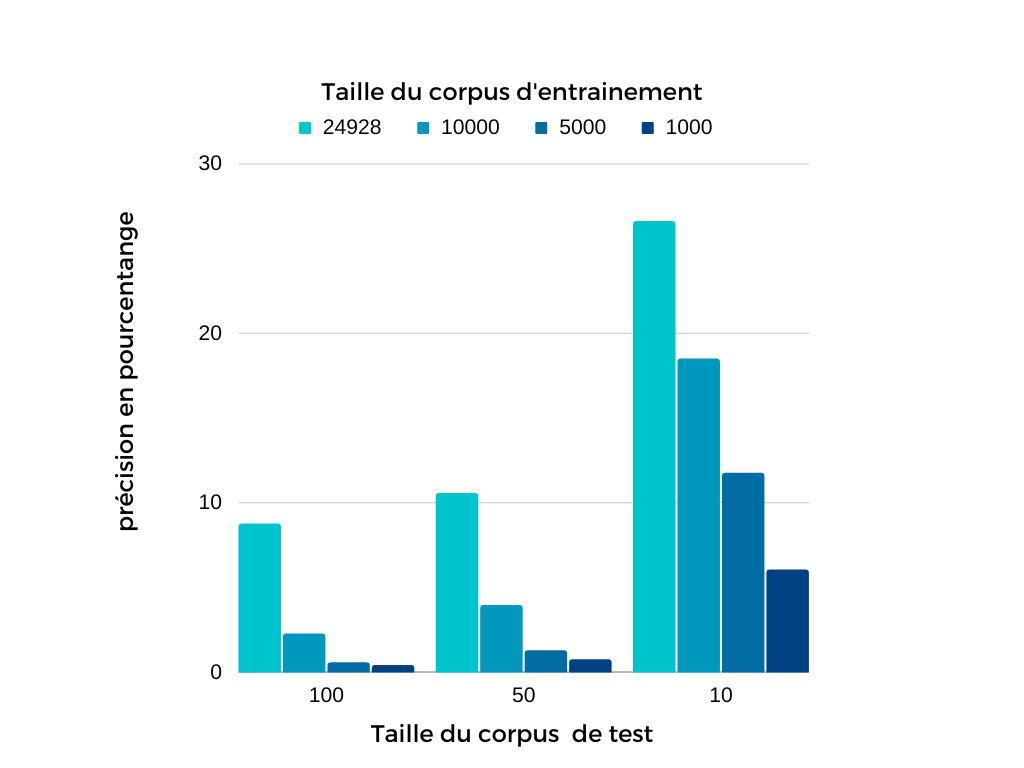
\includegraphics[scale=0.4]{img/TableauPrecision.png}
\caption{Graphique de la précision du classificateur}
\end{figure}


\end{center}
\newpage
\subsection{Comparaison}
Nous avons lancer la comparaison (jaccard, cosinus, et difflib) sur différents fichiers textes de différentes tailles (500, 1000 et 2000 mots ), avec un nombre de mots retirés/remplacés (croissant).\\
Voici les résultats obtenu:
(A noter que les résultats peuvent être très différents d'un fichier texte à un autre)\\

\begin{center}
\begin{figure}[h][t!]
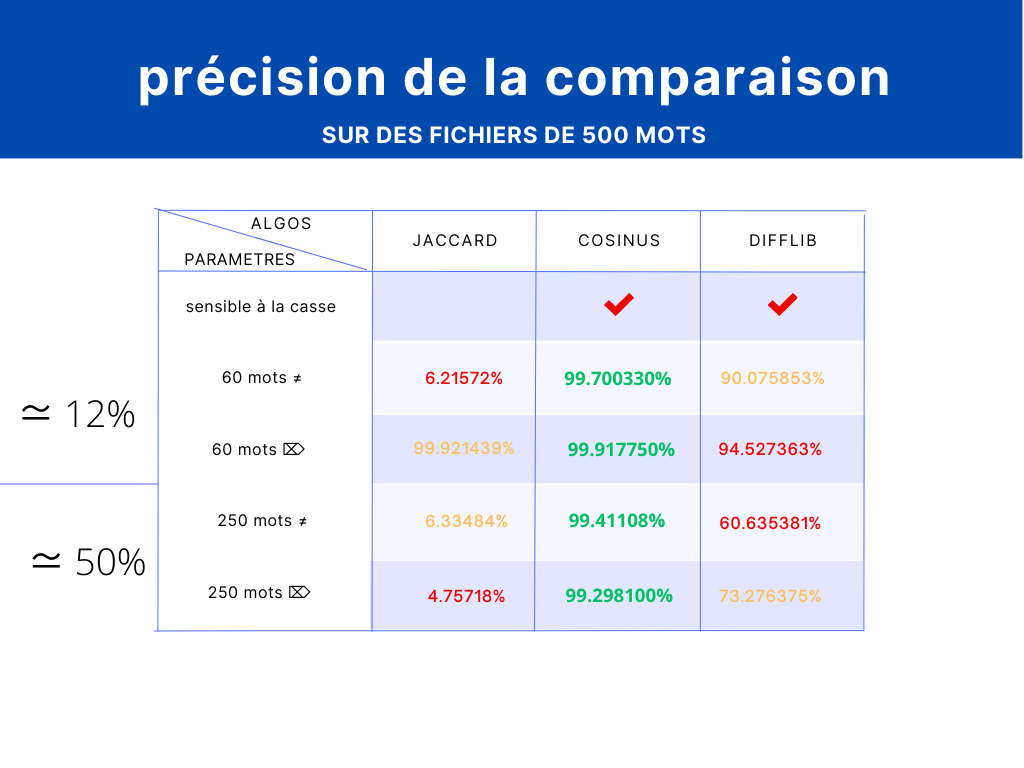
\includegraphics[scale=0.4]{img/jaccard_500_split.png}
\caption{exécution sur des fichiers de 500 mots}
\end{figure}


\end{center}
\begin{center}
\begin{figure}[h]
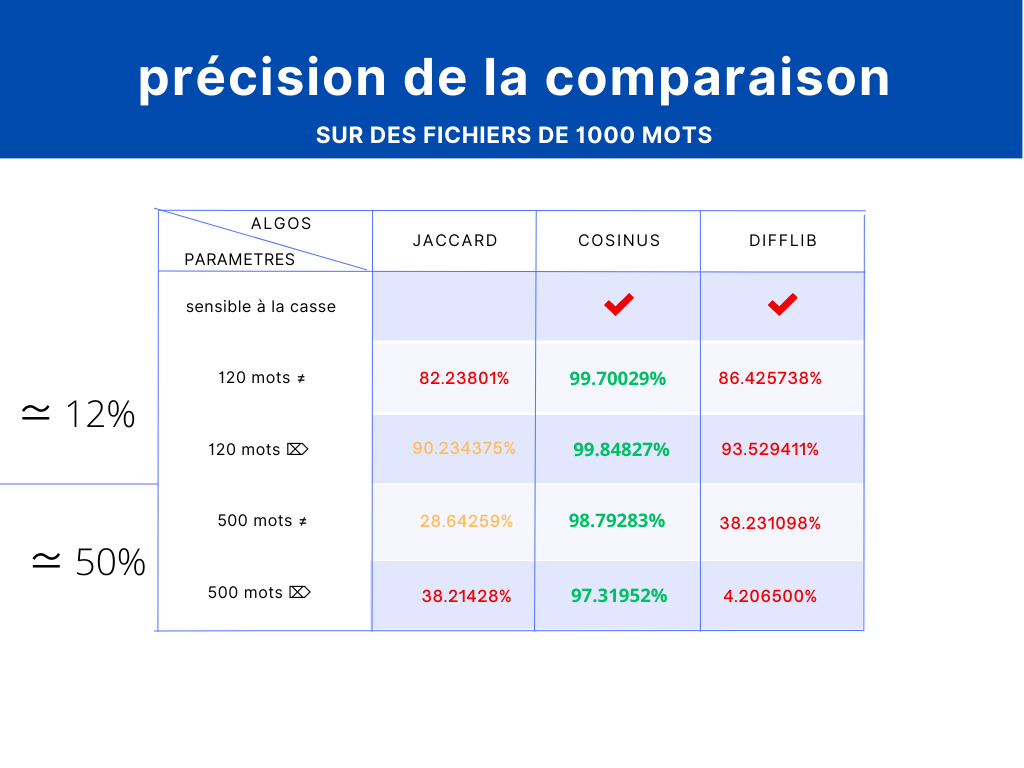
\includegraphics[scale=0.4]{img/true_jaccard_split_1000.png}
\caption{exécution sur des fichiers de 1000 mots}
\end{figure}


\end{center}

\begin{center}
\begin{figure}[ht!]
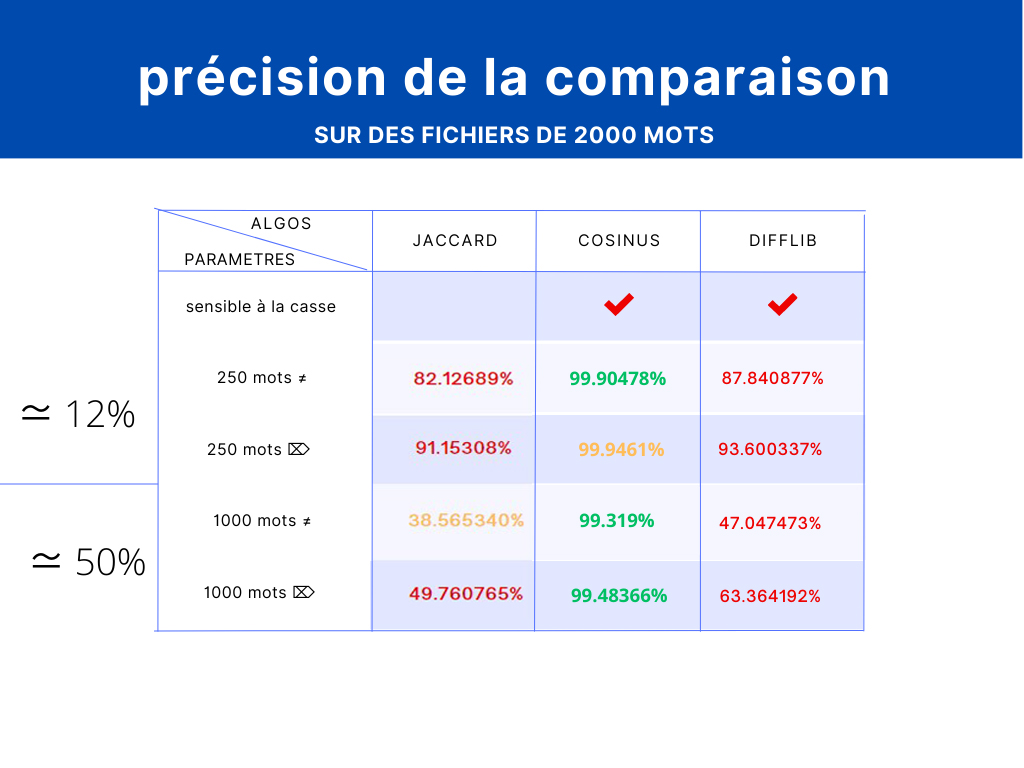
\includegraphics[scale=0.4]{img/true_comparaison_2000_mots.png}
\caption{exécution sur des fichiers de 2000 mots}
\end{figure}


\end{center}
\newpage
\section{Analyse des résultat}
\subsection{Classification}
D'après les expérimentations faîtes sur le classificateur de bayes on peut en déduire deux choses :\\

\begin{itemize}
	\item La première, on voit que la précision et l'efficacité augmente lorsque la taille du corpus de test diminue.
	\item La deuxième, on voit que la précision et l'efficacité diminue lorsque la taille du corpus d'entraînement diminue.\\
\end{itemize}

On peut donc en conclure que l'utilisation optimale du classificateur est avec un grand corpus d'entraînement et un petit corpus de test. De plus, plus les tailles des corpus d'entraînement et de test sont grandes, plus le classificateur mets du temps.\\
\subsection{Comparaison}
Il faut tout à bord savoir que les résultats ci dessus sont spécifiques au texte choisi, les résultats peuvent être différents à  environ  6\% selon les différents textes, cela est du notamment à  la fréquence des éléments de chaque texte, mais aussi des mots utilisés.
On peut tout de même en conclure certaines choses:
\begin{itemize}
    \item La méthode de \textbf{Jaccard} est simple à calculer et est  efficace pour des ensembles de données de petite à moyenne taille.
    Cependant, elle ne prend pas en compte la fréquence des éléments dans les ensembles, ce qui peut la rendre moins efficace pour des ensembles de données de grande taille ou pour des ensembles avec une forte variabilité de la fréquence des éléments.
    \item La méthode du \textbf{cosinus} retourne un résultat compris entre -1 et 1. Un score de similarité de 1 indique une correspondance parfaite entre les deux vecteurs de données, tandis qu'un score de similarité de -1 indique une complète différence entre les deux vecteurs. \\
    Un score de similarité de 0 indique que les deux vecteurs sont orthogonaux et n'ont aucune similarité.
    En pratique, pour des ensembles de données textuelles, les scores de similarité obtenus avec la méthode du cosinus sont souvent compris entre 0 et 1, car les vecteurs de mots sont rarement parfaitement opposés. Les scores de similarité proches de 0 indiquent que les documents sont peu similaires, tandis que les scores de similarité proches de 1 indiquent que les documents sont très similaires., 
     Cette méthode prend en compte la fréquence des éléments dans les vecteurs et est plus efficace pour des ensembles de données de grande taille ou pour des ensembles avec une forte variabilité de la fréquence des éléments( ce qui n'est pas le cas pour nous qui testons sur max 1000 mots différents).
    \item La méthode de \textbf{Difflib} qui est une bibliothèque de Python3 qui se base sur l'algorithme de Levenshtein, peut être utile pour des tâches de comparaison de chaînes de caractères de petite ou moyenne taille, mais elle peut être moins efficace pour des séquences de grande taille ou pour des séquences avec une grande variabilité de la fréquence des éléments. Elle est également sensible à la casse et à la ponctuation, ce qui peut affecter la précision de la mesure de similarité.
    
\end{itemize}


\section{Conclusion} \label{conclusion}
Nous avons donc une application web d'analyse de plagiat avec expérimentations complètes, c'était bien l'objectif que nous nous étions fixés.
Nous avons implémenté un classificateur fonctionnel ainsi que plusieurs algorithmes de comparaison et nous fait des expérimentations dessus afin de répondre à la problématique qui nous été posé.
En améliorations, nous aurions pu implémenté un deuxième classificateur afin de pouvoir faire une comparaison avec celui de bayes.

\section{Remerciements}
Nous souhaitons adresser nos remerciements les plus sincères à Monsieur Marc Spaniol pour son aide apportée, grâce à qui nous avons pu mener à bien ce projet ainsi que le rapport associé.\\
Nous remercions également Monsieur Bonnet Gregory, pour les explications et directives données lors des cours magistraux.\\

A tous ces intervenants, nous présentons nos remerciements, notre respect et notre gratitude.

\newpage

\end{document}